%%%%%%%%%%%%%%%%%%%%%%%%%%%%% Define Article %%%%%%%%%%%%%%%%%%%%%%%%%%%%%%%%%%
\documentclass{article}
%%%%%%%%%%%%%%%%%%%%%%%%%%%%%%%%%%%%%%%%%%%%%%%%%%%%%%%%%%%%%%%%%%%%%%%%%%%%%%%

%%%%%%%%%%%%%%%%%%%%%%%%%%%%% Using Packages %%%%%%%%%%%%%%%%%%%%%%%%%%%%%%%%%%
\usepackage{geometry}
\usepackage{graphicx}
\usepackage{amssymb}
\usepackage{amsmath}
\usepackage{amsthm}
\usepackage{empheq}
\usepackage{mdframed}
\usepackage{booktabs}
\usepackage{lipsum}
\usepackage{graphicx}
\usepackage{color}
\usepackage{psfrag}
\usepackage{pgfplots}
\usepackage{bm}
%%%%%%%%%%%%%%%%%%%%%%%%%%%%%%%%%%%%%%%%%%%%%%%%%%%%%%%%%%%%%%%%%%%%%%%%%%%%%%%

% Other Settings

%%%%%%%%%%%%%%%%%%%%%%%%%% Page Setting %%%%%%%%%%%%%%%%%%%%%%%%%%%%%%%%%%%%%%%
\geometry{a4paper}

%%%%%%%%%%%%%%%%%%%%%%%%%% Define some useful colors %%%%%%%%%%%%%%%%%%%%%%%%%%
\definecolor{ocre}{RGB}{243,102,25}
\definecolor{mygray}{RGB}{243,243,244}
\definecolor{deepGreen}{RGB}{26,111,0}
\definecolor{shallowGreen}{RGB}{235,255,255}
\definecolor{deepBlue}{RGB}{61,124,222}
\definecolor{shallowBlue}{RGB}{235,249,255}
%%%%%%%%%%%%%%%%%%%%%%%%%%%%%%%%%%%%%%%%%%%%%%%%%%%%%%%%%%%%%%%%%%%%%%%%%%%%%%%

%%%%%%%%%%%%%%%%%%%%%%%%%% Define an orangebox command %%%%%%%%%%%%%%%%%%%%%%%%
\newcommand\orangebox[1]{\fcolorbox{ocre}{mygray}{\hspace{1em}#1\hspace{1em}}}
%%%%%%%%%%%%%%%%%%%%%%%%%%%%%%%%%%%%%%%%%%%%%%%%%%%%%%%%%%%%%%%%%%%%%%%%%%%%%%%

%%%%%%%%%%%%%%%%%%%%%%%%%%%% English Environments %%%%%%%%%%%%%%%%%%%%%%%%%%%%%
\newtheoremstyle{mytheoremstyle}{3pt}{3pt}{\normalfont}{0cm}{\rmfamily\bfseries}{}{1em}{{\color{black}\thmname{#1}~\thmnumber{#2}}\thmnote{\,--\,#3}}
\newtheoremstyle{myproblemstyle}{3pt}{3pt}{\normalfont}{0cm}{\rmfamily\bfseries}{}{1em}{{\color{black}\thmname{#1}~\thmnumber{#2}}\thmnote{\,--\,#3}}
\theoremstyle{mytheoremstyle}
\newmdtheoremenv[linewidth=1pt,backgroundcolor=shallowGreen,linecolor=deepGreen,leftmargin=0pt,innerleftmargin=20pt,innerrightmargin=20pt,]{theorem}{Theorem}[section]
\theoremstyle{mytheoremstyle}
\newmdtheoremenv[linewidth=1pt,backgroundcolor=shallowBlue,linecolor=deepBlue,leftmargin=0pt,innerleftmargin=20pt,innerrightmargin=20pt,]{definition}{Definition}[section]
\theoremstyle{myproblemstyle}
\newmdtheoremenv[linecolor=black,leftmargin=0pt,innerleftmargin=10pt,innerrightmargin=10pt,]{problem}{Problem}[section]
%%%%%%%%%%%%%%%%%%%%%%%%%%%%%%%%%%%%%%%%%%%%%%%%%%%%%%%%%%%%%%%%%%%%%%%%%%%%%%%

%%%%%%%%%%%%%%%%%%%%%%%%%%%%%%% Plotting Settings %%%%%%%%%%%%%%%%%%%%%%%%%%%%%
\usepgfplotslibrary{colorbrewer}
\pgfplotsset{width=8cm,compat=1.9}
%%%%%%%%%%%%%%%%%%%%%%%%%%%%%%%%%%%%%%%%%%%%%%%%%%%%%%%%%%%%%%%%%%%%%%%%%%%%%%%

%%%%%%%%%%%%%%%%%%%%%%%%%%%%%%% Title & Author %%%%%%%%%%%%%%%%%%%%%%%%%%%%%%%%
\title{Ejercicio 34}

%%%%%%%%%%%%%%%%%%%%%%%%%%%%%%%%%%%%%%%%%%%%%%%%%%%%%%%%%%%%%%%%%%%%%%%%%%%%%%%

\begin{document}
\begin{figure}[ht]
    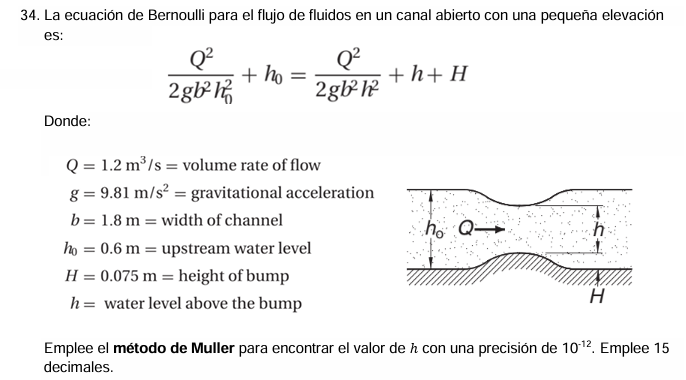
\includegraphics[scale=0.8]{img/mul34_1.png}
\end{figure}
 
Inciaremos declando las variables en matlab, de manera que:

$
q=1.2;
g=9.81;
b=1.8;
h0=0.6;
H=0.075;
$

Debemos llevar la ecuacion $\frac{Q^2}{2gb^2h_0^2}+h_0=\frac{Q^2}{2ggb^2h^2}+h+H$ a la forma $f(x)=0$. Por lo tando, la despejamos todo de un solo lado, asi:
\\$\frac{Q^2}{2gb^2h^2}-\frac{Q^2}{2gb^2h_0^2}+h+H-h_0=0$
\\Lo llevamos a matlab de forma $fx=((q^2)/(2*g*b^2*x^2))-((q^2)/(2*g*b^2*h0^2))+x-h0+H$


\noindent \\Vamos a graficar para determinar las raices:
\begin{figure}[ht]
    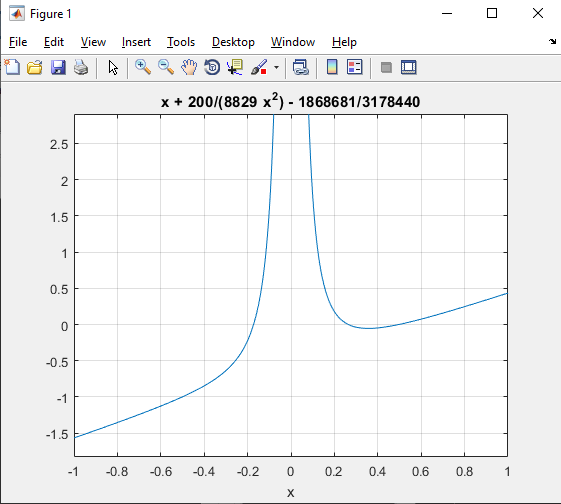
\includegraphics[scale=0.5]{img/mul34_2.png}
\end{figure}
\\No podemos tener un -h, por lo tanto podemos determinar que nuestra raiz se puede encontrar entre [0.2,0.3]

\noindent Seleccionaremos nuestros valores iniciales de manera que: $x0=0.21; x1=0.23; x2=0.25$. 
Ejecutemos el programa en Matlab para obtener el resultado.
\begin{figure}[ht]
    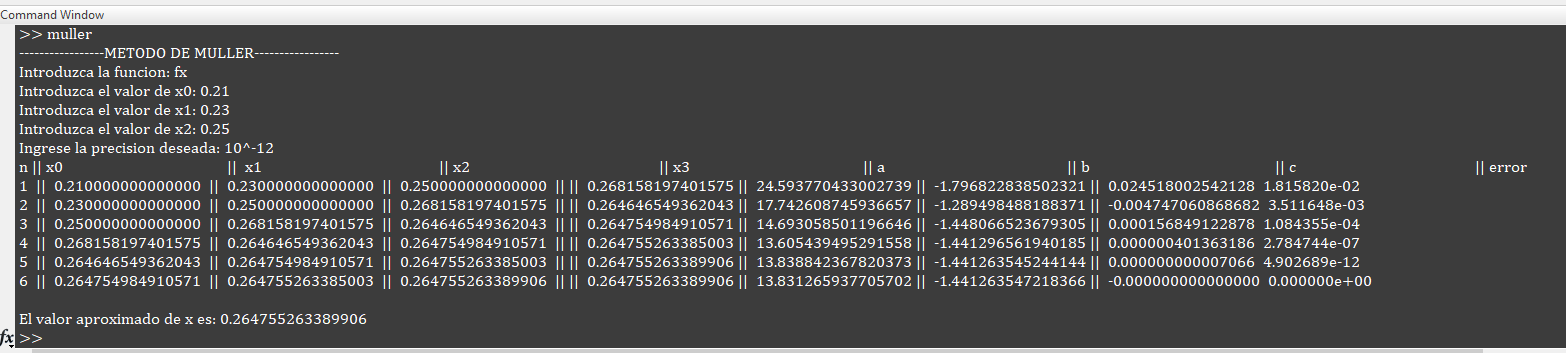
\includegraphics[scale=0.6]{img/mul34_3.png}
\end{figure}
\\El valor de h= 0.264755263389906
\\Ahora, existe un caso particiular en este ejercicio, si revisamos nuevamente el grafico podremos notar que la ecuacion tiene dos raices
\begin{figure}[ht]
    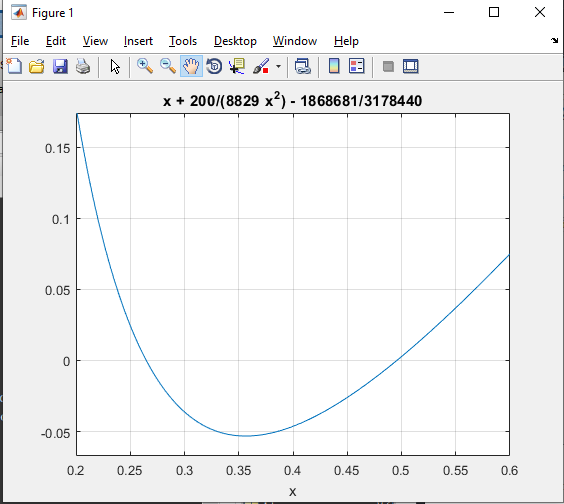
\includegraphics[scale=0.6]{img/mul34_4.png}
\end{figure}
\\Por lo tanto, calcularemos tamien su raiz para el intervalo [0.45,0.55]. Los punto a utilizar seran: $x0=0.47; x1=0.50; x2=0.53$
Calculemos ahora en matlab.
\pagebreak
\begin{figure}[ht]
    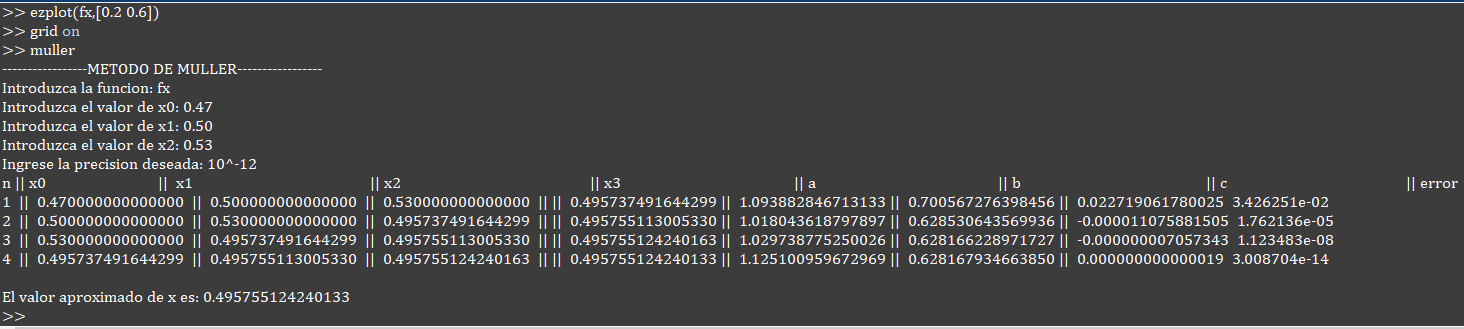
\includegraphics[scale=0.6]{img/mul34_5.png}
\end{figure}
\\La segunda raiz es h=0.495755124240133.
\end{document}